% "{'classe':('PSI'),'chapitre':'dyn_cin','type':('application'),'titre':'Pendule', 'source':'','comp':('C1-05','C2-09'),'corrige':False}"
%\setchapterimage{bandeau}
\chapter*{Application \arabic{cptApplication} \\ 
Pendule -- \ifprof Corrigé \else Sujet \fi}
\addcontentsline{toc}{section}{Application \arabic{cptApplication} : Pendule -- \ifprof Corrigé \else Sujet \fi}

\iflivret \stepcounter{cptApplication} \else
\ifprof  \stepcounter{cptApplication} \else \fi
\fi

\setcounter{question}{0}
\marginnote{}
\marginnote[1cm]{
\UPSTIcompetence[2]{C1-05}
\UPSTIcompetence[2]{C2-09}
}
%\begin{marginfigure}[4cm]
%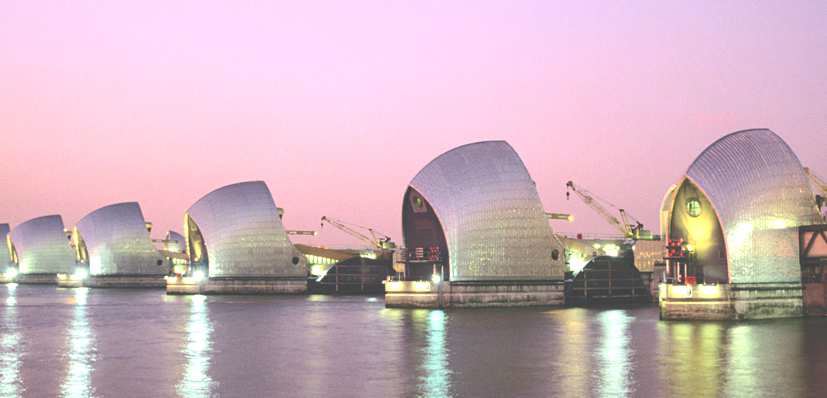
\includegraphics[width=\linewidth]{fig_00}
%\end{marginfigure}



\subsection*{Mise en situation}
On s'intéresse à un pendule guidé par une glissière. On fait l'hypothèse que le problème est plan. 

\begin{marginfigure}
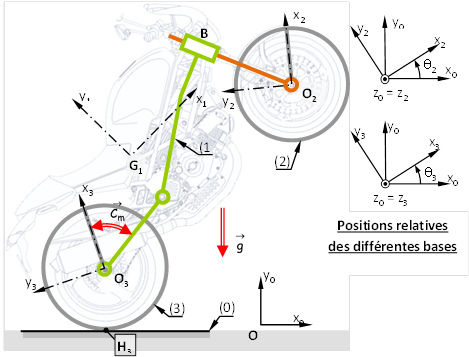
\includegraphics[width=\linewidth]{fig_01}
\end{marginfigure}

\begin{itemize}
\item On note 1 la pièce de masse $M_1$ et de centre de gravité $G_1$. $\vect{OA}=\lambda(t)\vect{x_0}-h\vect{y_0}$.
\item On note 2 la pièce de masse $M_2$ et de centre de gravité $G$ et de matrice d'inertie $\inertie{1}{G}= \matinertie{A}{B}{C}{-D}{-E}{-F}{\bas{2}}$. On a $\vect{AG}=L\vect{x_2}$
\end{itemize}

\subsection*{Travail à réaliser}

\question{Déterminer $\vectmd{A}{2}{0}$ en utilisant deux méthodes différentes. }
\ifprof
\begin{corrige}
~\\

\textbf{Cinématique}

On a $\vectv{G}{2}{0}=\deriv{\vect{OG}}{\rep{0}} $ 
$=\deriv{\lambda\vect{x_0}-h\vect{y_0}+L\vect{x_2}}{\rep{0}}$ 
$=\dot{\lambda}(t)\vect{x_0}+L\dot{\theta}\vect{y_2}$.



On a $\vectg{G}{2}{0}=\deriv{\vectv{G}{2}{0}}{\rep{0}} $ 
$=\ddot{\lambda}(t)\vect{x_0}+L\ddot{\theta}\vect{y_2}-L\dot{\theta}^2\vect{x_2}$.

\textbf{Cinétique \& dynamique}


On a $\vectmd{G}{2}{0} = \deriv{\vectmc{G}{2}{0}}{\rep{0}} $
\end{corrige}
\else
\fi



\question{En déduire le torseur dynamique $\torseurdyn{2}{0}$. }
\ifprof
\begin{corrige}
\end{corrige}
\else
\fi


\question{Isoler 2 et écrire le théorème du moment dynamique en $A$ en projection sur $\vz{0}$. }
\ifprof
\begin{corrige}
\end{corrige}
\else
\fi


\ifprof
\else
\begin{marginfigure}
\centering

\includegraphics[width=3cm]{Cy_04_02_Application_04_Pendule_qr}
\end{marginfigure}
\fi

\question{Isoler \{1+2\} et écrire le théorème de la résultante dynamique en  projection sur $\vx{0}$. }
\ifprof
\begin{corrige}
\end{corrige}
\else
\fi

